\documentclass[10pt,a4paper]{report}
\usepackage[utf8]{inputenc}
\usepackage[T1]{fontenc}		% Allow underscore in text
\usepackage[english]{babel}
\usepackage{amsmath}
\usepackage{amsfonts}
\usepackage{amssymb}
\usepackage{graphicx}
\usepackage[backend=biber,firstinits=true,sorting=none]{biblatex}
\usepackage{csquotes}
\usepackage{siunitx}
\usepackage{subcaption}
\usepackage{listings}
\usepackage{tikz}
\usepackage{tikzscale}
\usepackage{pgfplots}
\usepackage{color}
\usepackage{titlesec}
\usepackage{blindtext}
\usepackage{bm}

\graphicspath{ {figures/} }

\usetikzlibrary{positioning}
\tikzset{
	rect/.style={
	rectangle,
	minimum size=6mm,
	very thick,
	draw=white!20!black!80,
	top color=white,
	bottom color=white!50!black!20,
	% font=\itshape
	}
}

\pgfplotsset{compat=1.9}

\definecolor{codegreen}{rgb}{0,0.6,0}
\definecolor{codegray}{rgb}{0.5,0.5,0.5}
\definecolor{codepurple}{rgb}{0.58,0,0.82}
\definecolor{backcolour}{rgb}{0.95,0.95,0.92}
\definecolor{codeorange}{rgb}{0.95,0.45,0}
\lstdefinestyle{mystyle}{
    backgroundcolor=\color{backcolour},   
    commentstyle=\color{codegreen},
    keywordstyle=\color{magenta},
    numberstyle=\tiny\color{codegray},
    stringstyle=\color{codeorange},
    % basicstyle=\footnotesize,
    basicstyle=\ttfamily\small,
    breakatwhitespace=false,         
    breaklines=true,                 
    captionpos=b,                    
    keepspaces=true,                 
    numbers=left,                    
    numbersep=5pt,                  
    showspaces=false,                
    showstringspaces=false,
    showtabs=false,                  
    tabsize=2
}
\lstset{style=mystyle}

\definecolor{gray75}{gray}{0.75}
\newcommand{\hsp}{\hspace{20pt}}
\titleformat
	{\chapter}			% command
	[hang]				% shape
	{\Huge\bfseries}	% format
	{\thechapter\hsp\textcolor{gray75}{|}\hsp} % label
	{5pt}				% sep
	{\Huge\bfseries}	% before code


\author{André Hedlund}
\title{Effective Finite Element Analysis Workflow for Structural Mechanics}

\bibliography{thesis.bib}

\begin{document}
\maketitle
%\begin{abstract}
%\end{abstract}
\tableofcontents

%!TEX root = report.tex

\chapter{Introduction}
\label{cha:introdution}
% \subsection{Hydro-Electric Power}
Hydro-power is the worlds largest renewable energy source, and hydroelectric power plants have been developed and used since the nineteenth century. During the last decade hydro-power amount to 45 percent of the total electricity production in Sweden~\cite{scb}. Many of the hydro-power plants in Sweden were built several decades ago, and they are therefore in need of refurbishment and modernisation. A simplified description of a conventional hydro power plant is that it consist of a dam, turbine and a generator, where the dam creates a water reservoir that contains potential energy that drives the turbine which in turn generates electricity.

% \subsection{Andritz Hydro}
The Andritz Group provides services mainly for the hydro-power, pulp and paper, and metals industries, with headquarters in Graz, Austria and approximately \num{24500} employees worldwide. Andritz Hydro is a supplier of electromechanical equipment for hydro-power plants, and the Swedish subsidiary Andritz Hydro AB (henceforth referred to as Andritz) has 160 employees and focuses mainly on refurbishment and optimisation of turbines and generators.

% Write about the 'product realization process'
At Andritz the entire product development process is performed, including product design, analysis and manufacturing. The design process, usually referred to as CAD (Computer Aided Design), and the analysis process, usually referred to as CAE (Computer Aided Engineering), are the parts of the product development that is the focus of this thesis.

Turbines and generators are advanced electromechanical equipment, and since hydroelectric power plants need to reliably operate under long terms, the modernisation process is subject to rigorous analysis to ensure long term operation. Therefore, it is important to analyse the structure's capability to support the applied loads; \textit{structural mechanics} focuses on the computation of deformations and stresses, to evaluate the performance of the structure. The physical phenomena that are investigated (stress, strain, deformation, etc.) are modelled by solving differential equations together with a set of boundary conditions. Generally, there exist no analytical solutions to differential equations that relate to complex structures, therefore, the only way to estimate solutions of the equations are with numerical methods.

The finite element method (FEM) is a numerical approach that can be used to approximate the solution of boundary value problems. The method has been used rigorously in different engineering disciplines for several decades, and its main advantage over other numerical methods for solving differential equations is its capability to handle complex geometries. The structure is divided into smaller parts, called elements, which together create a discrete mesh that represent the geometry.~\cite{ottossen92}

% Write about why the workflow is problematic at Andritz
There exist several different software programs for CAD and CAE, at Andritz \textit{Siemens NX} is used for CAD and \textit{Salomé} together with \textit{Code Aster} are used for the finite element analysis (FEA). The analysis process is comprised of three steps: pre-processing, solution and post-processing. The goal of the pre-processing is to from a CAD model develop an FE model containing a mesh, material definitions and boundary conditions. In general, a significant amount of time is spent on the pre-processing and a lot of manual work can be required by the analyst, it is therefore important to make the pre-processing as effective as possible.

At Andritz the analysis workflow is in some aspects cumbersome and convoluted, and a more streamlined workflow is desired. Some of the difficulties occur solely because of that two different software programs are used for CAD and CAE, and other difficulties are generically inherited from the software programs that are used.

The purpose of this thesis is to evaluate the current workflow at Andritz, based on time-efficiency and convenience. Based on what the evaluation manifest, suggestions to improve the workflow will be presented. The suggestions are concerned with both larger strategical improvements, such as evaluating other software programs, and smaller improvements that simplify time-consuming repetitive processes. The main aspects to consider are:
\begin{itemize}
	\item time-efficiency,
	\item simple and convenient processes,
	\item cost-efficiency and
	\item easy and fast to learn.
\end{itemize}

Since the product development process is complex, it is not certain that there exist feasible solutions that improves the workflow. It is also not guaranteed that the software programs provides functionality such that processes can be simplified.


%\subsection{Finite Element Analysis}
%
%\subsection{Finite Element Analysis at ANDRITZ} \label{sec:feaandritz}
%
%When a part is subject to an analysis the calculation engineer start with a part in NX. The part is idealised by removing smaller holes, chamfers and fillets that are non-essential for the analysis. Idealising the part can be done with the synchronous modelling commands that are available in NX. The part is now exported as a \texttt{.step} file that contains the geometrical description of the part.
%
%The \texttt{.step} file is imported into Salome-Meca a software platform for pre- and postprocessing. The idealisation that is done in NX is the first step in the preprocessing of the part. The next step is to create the necessary groups where boundary conditions and loads will be applied. The final step of the preprocess is to mesh the part, the part needs to be divided into a set of elements that describe the original model in accurately. The part is now exported from Salome-Meca, a text file that describes the geometry, the mesh and the defined groups is produced.
%
%The next part of the analyses is to solve the case by first defining the boundary conditions, load cases and physical properties that are needed to create a tractable model. These steps are done with command-line driven open source FEM package called Code Aster. The text file that Salome-Meca produced describes the geometry, mesh and groups that adheres to the \texttt{.unv} format, this format is not preferred by Code Aster, therefore the \texttt{.unv} file is converted to a \texttt{.mail} file. The case setup is described in a \texttt{.comm} file that is read by Code Aster.
%
%The post-processing is performed in Salome-Meca where the results created by Code Aster is imported. The final analysis of the results are visualised as needed.
%
%\begin{figure}
%	\centering
%	\rule{2cm}{2cm}
%	\label{fig:workflow}
%	\caption{A schematic figure of the workflow at Andritz for finite element analyses.}
%\end{figure}
%
%\subsection{Goal}
%The main focus of this thesis is to investigate the possibility to imporove this workflow process, to see if any changes are possible and if they would improve efficiency. There are several perspectives that could be investigated, and the main focus of this thesis will be on:
%\begin{itemize}
%	\item NX provides a utility called \emph{Advanced Simulation} that includes the functionality to both create groups and mesh from NX. If \emph{Advanced Simulation} fulfils the requirements of the current process, it would be possible to eliminate several steps from the workflow that is described in section~\ref{sec:feaandritz} and Figure~\ref{fig:workflow}.
%	\item \emph{Advanced Simulation} also includes the functionality to use some of the eminent solvers Nastran, Abaqus and Ansys. Therefore it is of interest to investigate how this functionality works in NX.
%\end{itemize}
%Eventhough the focus of the investigation is to evaluate the technical functionalities of NX and \emph{Advanced Simulation}, it is important to establish that the current NX license that is used at Andritz does not include the \emph{Advanced Simulation} utility. Therefore, the investigated paths described above would result in an increase of the costs, since the current softwares (Salome-Meca and Code Aster) are open source and free of charge.
%
%The investigation will also take another perspective, which is to try and improve the current workflow, without changing any of the main steps. The current workflow contains several exports and imports between different softwares and a general analysis could include several iterations between the calculation team and the design team. During these iterations, small, but significant changes are made on the part that is under analysis. Due to the convoluted workflow it is difficult to reuse the settings and work done on the previous part, therefore the process has to be repeated even if just a small change has been done to the part. This is particularly evident in the preprocessing step in Salome-Meca, where the defined groups and mesh settings are lost between these iterations. 
%
%Salome-Meca provides a python API (Application Programming Interface) such that the user might create its own scripts to perform tasks that are not provided by Salome-Meca. With this functionality it is possible to investigate if a script can be written such that it can compare the part from the previous iteration with the new part to see if some of the groups and meshes can be copied to the new part. If this is possible then it would eliminate the nuisance of having to recreate the settings between the iterations.
%
%
%






%!TEX root = report.tex

\chapter{Theory} % (fold)
\label{cha:theory}
This section gives a basic introduction to the Finite Element Method (FEM) for structural mechanics, and describes the different stages of finite element analysis (FEA). It also presents the software programs that are used in the current analysis workflow at Andritz Hydro AB.

\section{Finite Element Method for Structural Mechanics} % (fold)
\label{sec:finite_element_method_in_structural_mechanics}
Here follows a short but descriptive text about FEM.
When, where and why did it originate?
Elements
Mathematical formulation
System of equations

During the design of structures it is important to analyse the structure's capability to support the applied loads; structural mechanics focuses on the computation of deformations and stresses, to evaluate the performance of the structure. The physical phenomena that are investigated (stress, strain, elasticity etc.) are modelled by differential equations together with a set of boundary conditions. Generally, there exist no analytical solutions to differential equations that relate to complex structures, therefore, the only way to solve the equations are with numerical methods.

The finite element method is as numerical approach that can be used to approximate the solution of boundary value problems. The method has been used rigorously in different engineering disciplines for several decades, and its main advantage over other numerical methods for solving differential equations is its capability to handle complex geometries. The structure is divided into smaller parts, called elements, which together create a discrete mesh of the geometry.~\cite{ottossen92}

(Maybe add section with mathematical FEM description. degrees of freedom)

\subsection{Pre-Processing} % (fold)
\label{sub:pre_processing}
When a structure has been designed, the CAD model needs to be analysed to determine if the desired performance qualifications are reached. The first step of the analysis is the pre-processing, which is the step that prepares the model for a computation.

% Clean: FEA book p. 181-191
Ideally, the CAD model built by the design team is usable for finite element analysis without having to alter the model. However, this is often not the case, since it often exists features that are problematic from an analysis viewpoint. Therefore, it is necessary to make simplifications to the model in order to create a mesh of the model. Design features that complicate automatic meshing are short edges, sliver faces, small holes, fillets, chamfers etc., and it is necessary to clean the model of these features to enable the automesher to mesh the model. This cleaning process can be both tedious and difficult since it may exist a lot of features, and even if a disadvantageous feature is found it may be difficult to remove it; the cleaning process can therefore be very time consuming. It is also important to mention that the simplifications that is performed should not influence the structural capabilities of the model, this could be difficult to assess, but as long as the simplifications are local and not in areas of interest the structural capabilities should not be affected.~\cite[p.~181--191]{adams99}

% Meshing
When the model is clean, the next step is to mesh the model. Whether the model is meshed automatically or manually and with shell elements or tetrahedrons, the process is an essential step of the analysis. The focus of this thesis is on automeshing with tetrahedrons (for 3D models) and triangles (for 2D models). Automeshing is a simple and efficient technique to create a discrete FE model of the CAD model. Depending on which automesher that is used different settings are available, but the user should generally consider the maximum and minimum elements size, element growth rate and local mesh refinements. The goal is to create a mesh that captures the structural features of the model with as few elements as possible. Even though the automesher could create the mesh in a fast and convenient way, it is no guarantee that the mesh is sufficiently refined. Therefore, considerable thought should be spent on where local mesh refinements are necessary, how small elements are needed and how large elements are excepted. It is also important to mention that it is an absolute necessity that the model is clean, otherwise the automesher will most likely fail to create a mesh.~\cite[p.~251-255]{adams99}

Part of the pre-process is also to define the boundary conditions that influence the model. There exist two groups of boundary conditions: constraints that prohibits the model from moving in the specified spatial degrees of freedom, and loads such as forces, moments and temperature. How the boundary condition are defined and which types that are used are often not straightforward, and an important part of the analysis.~\cite[p.~263]{adams99}

Before the FE model can be solved the material properties of the model needs to be specified.

It is probably obvious that this part of the analysis can be very time consuming, and to obtain a solution it is of paramount importance that the FE model is created correctly, with sufficient details of the original model and that boundary conditions are properly defined.
% subsubsection pre_processing (end)

\subsection{Solution} % (fold)
\label{sub:solution}
When the FE model is created, the next step is to solve the model to obtain the results. This step is mainly executed by the computer, the only effort from the user is setting the correct solver parameters. Which parameters that can be specified is highly dependent on which solver is used. The execution time depends on how large the FE model is (number degrees of freedom) and what solution type is used (non-linear solutions are more demanding).

When the solver is finished it is important to evaluate the results and the solver output to establish if the solution is reasonable and if the results are accurate. To determine if the mesh is sufficiently refined the convergence could be checked, and to check that the boundary conditions are properly defined the resultant forces on the model could be compared with the specified loads.~\cite[p.~303-324]{adams99}
% subsubsection solution (end)

\subsection{Post-Processing} % (fold)
\label{sub:post_processing}
The first step of the post-processing is to visualise the results (displacement, stress, etc.) to determine if the solution is reasonable. If the solution is reasonable the FE model can be considered to be adequate. The next step is to visualise the specific results that are the goal of the analysis. Even if this step is not very technical, it is important to analyse the results to determine if the results can be trusted.
% subsubsection post_processing (end)

\subsection{Elements} % (fold)
\label{sub:elements}
Describe different types of elements.
% subsubsection elements (end)

\subsection{Boundary Condidtions} % (fold)
\label{sub:boundary_condidtions}
Describe different types of bc's.
% subsubsection boundary_condidtions (end)

\subsection{Load Cases} % (fold)
\label{sub:load_cases}
Maybe not necessary
% subsubsection load_cases (end)

\subsection{Contacts} % (fold)
\label{sub:contacts}
Describe non-linearity, meshing technique etc.
% subsubsection contacts (end)

% subsection finite_element_method_in_structural_mechanics (end)

\section{Siemens NX} % (fold)
\label{sec:siemens_nx}
Write some general about NX and which features that are used. Also write about Advanced Simulation.

NX\texttrademark{} is a software developed by Siemens PLM Software that supports every aspect of product development (i.e. design, analysis and manufacturing)~\cite{siemensnx}. This section describes a subset of the functionality provided by NX that is relevant for this thesis, and the focus is on the tools to clean the model (called Synchronous Modelling  tools) and the analysis solution (called Advanced Simulation).~\cite[p.~36ff.]{goncharov14}

The synchronous modelling tools that are provided by NX are very efficient and powerful to use during the cleaning process. Synchronous modelling extends the regular parametric modelling approach that is used in CAD with more intuitive and direct modelling tools. The tools that are most commonly used are: \textit{Move Face}, \textit{Delete Face}, \textit{Make Coplanar}, \textit{Pull Face} etc., for a description of these tools see~\cite{goncharov14}. The main advantage of these tools is that the model can be changed without having access to the or making changes to the original history-tree of the commands that created the model.

NX Advanced Simulation provides the entire CAE workflow with pre- and post-processing and solver environment. It is also tightly integrated with the CAD application of NX, enabling a fast and efficient analysis process. The meshing capabilities that Advanced Simulation provides are the usual 3D and 2D automeshers as well as more exotic elements for specific applications. The simulation environment can be integrated with several of the most common solvers such as NX Nastran, Abaqus and Ansys.
% subsection siemens_nx (end)

\section{Salomé Platform} % (fold)
\label{sec:salom_platform}
Salomé is a free software platform (distributed under GNU LGPL~\cite{lgpl}) for numerical simulation. Salomé strives to provide a framework where the entire workflow of a numerical simulation (described in sec.~\ref{sub:pre_processing}-\ref{sub:post_processing}) can take place. The platform consists of different modules that can be used for pre- and post-processing, which are presented under the same GUI (graphical user interface).~\cite{ribes07} 

\subsection{Geometry Module} % (fold)
\label{sub:geometry_module}
The \textit{Geometry} module provides basic functionality to import CAD models and prepare them for numerical simulation. Common tasks that are carried out in this module is:
\begin{itemize}
 	\item create groups
 	\item partition objects
 	\item whateva
\end{itemize}

A group in Geometry is a collection of geometrical objects (solids, faces, edges or vertices), which is given a common name and can be referenced by that name from other modules. Groups are used for three different purposes: local mesh refinement, boundary conditions and contact surfaces.

To be able to control the automeshing it is useful to define patches on the model where local mesh refinements are necessary to get the solution to converge. A patch is a group of faces or edges that should be better resolved. Any geometrical object of the model that is the subject of a boundary condition should also be defined as a group. If two objects are in contact, and a contact simulation is required, the contact surfaces should be defined as groups.

The partition function connects solid objects and creates a single solid, but the contact face will still remain between the objects. This function is mainly used when a conformal mesh has to be created for a contact simulation.~\cite{salomedoc}
% subsubsection geometry_module (end)

\subsection{Mesh Module} % (fold)
\label{sub:mesh_module}
When a model has been imported to Geometry and and the groups are defined, the \textit{Mesh} module can mesh the model. Mesh provides the most common elements and several different algorithms for mesh generation are available, resulting in a very extensive library of functions.

To mesh an object with the Mesh module first an object from Geometry is selected, then an algorithm is selected and finally an hypothesis is created. The hypothesis represent the parameters that the algorithm use to create the mesh, depending on the algorithm different parameter values are specified in the hypothesis. Since there exist several algorithms in Mesh, this section only describes the \textit{NETGEN} algorithm and the \textit{Projection} algorithm.

The NETGEN algorithm~\cite{netgen} is an automesher that can be used for creating 3D tetrahedral meshes and 2D triangular and quadrilateral meshes. The hypothesis for the NETGEN algorithm specifies
\begin{itemize}
	\item the maximum and minimum element size, 
	\item if second order elements should be used,
	\item growth rate,
	\item the possibility to specify the number of elements based on surface curvature, and
	\item local refinements on specified groups. 
\end{itemize}

The projection algorithm creates a mesh of an object by projecting the mesh of another object. This algorithm is especially used when conformal meshes are desirable.

The mesh module supports, just as the Geometry module, the creation of groups. This feature is specifically useful when a specific part of the mesh needs to be referenced or exported.

\subsubsection{Contact Mesh} % (fold)
\label{ssub:contact_mesh}
If the analysis contains contacts, it is in some cases necessary to have matching meshes at the contact surface. A matching mesh means that the mesh of the two objects in contact have nodes at the same place at the contact surface.
% subsubsection contact_mesh (end)
% subsubsection mesh_module (end)

\subsection{ParaVis Module} % (fold)
\label{sub:paravis_module}
The ParaVis module is based on ParaView an open source platform for data analysis and visualisation. Suffice to say that all the functionality needed to visualise the results in a structural analysis is provided.
% subsubsection paravis_module (end)

\subsection{Application Programming Interface (API)} % (fold)
\label{sub:application_programming_interface_}
A very advantageous feature of Salomé and the modules that have been described is that the functionality provided by the GUI also is available through an API, enabling the user to write scripts that execute functions automatically.

An API is a framework of functions for building software applications. Using the API a developer can efficiently create software that perform specific tasks by using the functionality provided by the API. The documentation of the API describes which functions that are available and what each functions does.

Salomé's API is based on the Python programming language and the Salomé GUI includes a Python console, by which the user can execute scripts that utilise the API. There exist a specific API for each module and these can work together within the same script, therefore it is possible to write a script that first import a model to Geometry where groups are created, then the script can select an algorithm and create a hypothesis, and finally the script can update the GUI.

\begin{figure}[t]
	\begin{center}
		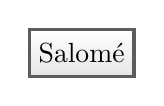
\begin{tikzpicture}
			\node[rect] (salome)	{Salomé}; 
		\end{tikzpicture}
	\end{center}
	\caption{Some schematic view of the Salomé platform}
	\label{fig:salome}
\end{figure}

% subsubsection application_programming_interface_ (end)

% subsection salom_platform (end)

\section{Code\_Aster} % (fold)
\label{sec:code_aster}
Code\_Aster~\cite{codeaster} is an open source FEM software for structural analysis which is developed by EDF (Électricité de France) and distributed under GPL (General Public License)~\cite{gpl}. The software is driven by an input file with commands that that describe the simulation (a COMM file), and a text file describing the mesh (usually a MAIL file). The information the MAIL file needs to contain is the mesh data, that is the nodes and the elements of the mesh, but the file also needs to describe the patches on which the boundary conditions are applied, these patches can be created in the Mesh module as described in Section~\ref{sub:mesh_module}. The output is text files describing general information about the simulation (errors, warnings, convergence, etc.) and a file containing the results which can be imported to Salomé and visualised with the ParaVis module. 
% subsection code_aster (end)

% section theory (end)

%!TEX root = report.tex

\section{Analysis} % (fold)
\label{sec:analysis}
The previous section described structural analysis and FEA in general and presented different software programs that can be used in the analysis. This section presents how FEA is performed at Andritz Hydro AB based on the investigation made by the author of this thesis. The investigation is the basis of the improvement suggestions that are given in this section.

\subsection{Analysis Workflow at Andritz} % (fold)
\label{sub:analysis_workflow_at_andritz}
% Product development process: FEA p. 12-13
The structural analysis begins with a CAD model created by the design team. The design engineers at Andritz Hydro AB use Siemens NX to create CAD models, internally in NX these models are called \textit{parts}. The parts are given a reference number to a database where they are stored, and this reference number is passed on to the calculation team. As described in Section~\ref{ssub:pre_processing}, the CAD model needs to be cleaned of features that are unnecessary to the analysis, since the cleaning process can change the model significantly, it is not appreciated by the design engineers that the model they created is altered, therefore, a copy of this model is created which can be prepared for analysis. A copy is created by creating a new part in the database that is assigned to the calculation engineer and then using a synchronous modelling tool to link the part created by the design engineer.

The cleaning process is done in NX with the synchronous modelling tools that is described in Section~\ref{sub:siemens_nx}. Depending on the detail level of the model that is provided, the amount of work that is needed on the cleaning process can range from very little to a significant part of the entire analysis process. 

When the part is ready to be meshed it is exported from NX. There exists several formats to export a CAD model such that the details of the model are preserved, and at Andritz the standard STEP (standard for the exchange of product model data) format is used. A STEP file describes a CAD model according to an ISO standard which is used for file exchange~\cite{stepiso}.

The rest of the pre-processing is carried out in the Salomé Platform described in Section~\ref{sub:salom_platform}. The STEP file is imported and the Geometry module is selected. As described in Section~\ref{ssub:geometry_module}, groups are created in the Geometry module to define where local mesh refinement is needed, where boundary conditions are applied and possible contact surfaces.

After the groups are defined the the analyst change to the Mesh module where the model is meshed. The meshing process in Salomé is described in Section~\ref{ssub:mesh_module}. 3D models are usually meshed with tetrahedrons (see Sec.~\ref{ssub:elements}) and 2D models are usually meshed with triangles, in both cases the NETGEN algorithm is used.

To solve the model Code Aster is used and, as is described in Section~\ref{sub:code_aster}, Code Aster requires the mesh to be described in a text file where patches, on which boundary conditions are applied, are defined. Therefore, mesh groups are defined in the Mesh module before the mesh is exported.

The final steps of the analysis has not been investigated to the same level of detail, and are therefore summarised just to describe the entire workflow of the analysis. When the file describing the mesh has been created, the COMM file that describes the simulation is written. This file describes the type of simulation, boundary conditions and other parameters depending on the type of simulation. The simulation is executed with these two input files and the output is the results that can be visualised and analysed with the ParaVis module. 

The workflow described is presented in Figure~\ref{fig:andritz_workflow}. 

\begin{figure}[t]
	\begin{center}
		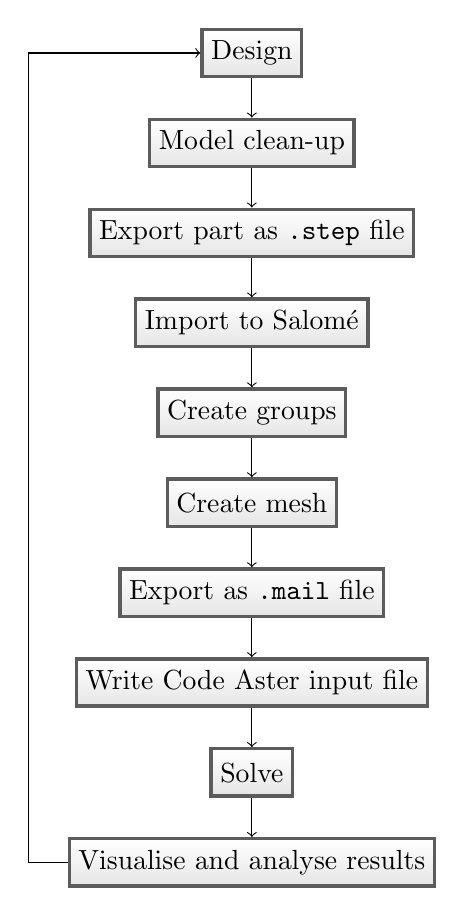
\begin{tikzpicture}[node distance=5mm]
			\node[rect] (design)					{Design};
			\node[rect] (clean)	[below=of design] 	{Model clean-up};
			\node[rect] (step)	[below=of clean]	{Export part as \texttt{.step} file};
			\node[rect] (salom)	[below=of step]		{Import to Salomé};
			\node[rect] (group) [below=of salom] 	{Create groups};
			\node[rect] (mesh)	[below=of group]	{Create mesh};
			\node[rect] (mail)	[below=of mesh]		{Export as \texttt{.mail} file};
			\node[rect] (comm)	[below=of mail]		{Write Code Aster input file};
			\node[rect] (solve)	[below=of comm]		{Solve};
			\node[rect] (vis)	[below=of solve]	{Visualise and analyse results};
			\path (design)	edge[->]	(clean)
				  (clean)	edge[->]	(step)
				  (step)	edge[->]	(salom)
				  (salom)	edge[->]	(group)
				  (group)	edge[->]	(mesh)
				  (mesh)	edge[->]	(mail)
				  (mail)	edge[->]	(comm)
				  (comm)	edge[->]	(solve)
				  (solve)	edge[->]	(vis);
			\draw [->] (vis.west) -- ++(-.5,0) |- (design.west);
		\end{tikzpicture}
	\end{center}
	\caption{Current analysis workflow at Andritz Hydro AB.}
	\label{fig:andritz_workflow}
\end{figure}

If the results are feasible the development of the CAD model can continue, and preparations for the manufacturing process can begin. However, if the results show that the model does not fulfil the requirements the model needs to be redesigned and the analysis repeated on the updated model. This iteration procedure is standard in product development. Since the analysis of the updated model is likely to be very similar to the original model some of the steps described in Figure~\ref{fig:andritz_workflow} are reusable, however, some steps have to be performed again. During the analysis of a redesigned model the following steps cannot be reused:
\begin{itemize}
	\item Model clean-up
	\item Create geometric groups
	\item Create mesh
	\item Create mesh groups
\end{itemize}
Obviously the visualisation and analysis of the results need to be repeated, but that is unavoidable. The four steps mentioned above are all part of the pre-process of the analysis, and they could be a very time consuming part of the analysis, so it would be favourable to find a solution that could reuse the fact that these steps already have been performed on a very similar model. 

It is also possible that half way through the analysis there could be an update to the original CAD model that is independent of the analysis. If the update is significant to the analysis a new analysis needs to be started in this case as well. This is because the link between the CAD model and the analysis model is broken during the first step when the CAD model is copied. This is obviously very frustrating and time consuming for the analyst. Since these updates of the CAD model are impossible to prevent a solution that diminish the effect of the update is very desirable.
% subsection analysis_workflow_at_andritz (end)

\subsection{Using NX Advanced Simulation} % (fold)
\label{sub:using_nx_advanced_simulation}
The previous section described the structural analysis workflow at Andritz Hydro AB and highlighting parts of the workflow that is inefficient, especially if a new iteration is started. This section describes a possible solution some of the problems that are discussed. NX Advanced Simulation (described in Sec.~\ref{sub:nx_advanced_simulation}) supports the entire analysis process 
% subsection using_nx_advanced_simulation (end)

\subsection{Salomé API Script} % (fold)
\label{sub:salom_api_script}

% subsection salom_api_script (end)




% section analysis (end)

%\input{discussion}

%!TEX root = report.tex

\chapter{Conclusions} % (fold)
\label{sec:conclusions}
This chapter discuss the different solutions presented in Chapter~\ref{cha:analysis}, and recommends the -- according to the author -- preferred workflow for FEA at Andritz. The two different approaches (NX Advanced Simulation and Salomé API Script) are first discussed separately and in the last section the final recommendation is presented.

\section{NX Advanced Simulation} % (fold)
\label{sec:nx_advanced_simulation}
With NX Advanced Simulation the entire FEA workflow can be performed within the same software, therefore eliminating the time spent on transferring files between different software programs. The environment that Advanced Simulation provides with the idealised part and the associativity to the original CAD model is very efficient for the design-analysis iterations. Advanced Simulation can therefore be expected to increase efficiency for the calculation engineers at Andritz.

There is currently only one Advanced Simulation license at Andritz (MasterFEM). There are at least three calculation engineers that need a license, therefore, additional licenses need to be purchased if Advanced Simulation should be used as CAE software. Since the solver is used in the background, whereas the pre- and post-processing features are used in the foreground by the user, it is possible to manage the workflow with a separate pre- and post-processing license for each calculation engineer and a shared solver license between the calculation engineers. Therefore it would suffice if the calculation team purchased three NX Advanced FEM licenses and kept the current NX Nastran solver, but since it might be too limited to only have one solver another possibility is to purchase one NX Advanced FEM and two NX Advanced Simulation licenses. These two different configurations represent a price range of \num{305760} -- \num{377720} SEK; this cost is an important aspect to consider with this particular workflow.

Since the calculation engineers at Andritz have been working with the Salomé Platform and Code Aster in their FEA, it is also expected that the introduction of a new solver and GUI (Graphical User Interface) will demand a learning curve that can be costly depending on the usability of Advanced Simulation. Even though the GUI is relatively easy to use and a comprehensible documentation exists, the time that is lost on learning the new software can be significant and it might even be necessary with training courses for the employees (that comes at an additional cost).

% section nx_advanced_simulation (end)

\section{Salomé API Script} % (fold)
\label{sec:salom_api_script_conclusions}
The current workflow (see Sec.~\ref{sec:analysis_workflow_at_andritz}) uses NX for cleaning, Salomé for meshing and defining where boundary conditions, etc. are applied, Code Aster for solving, and Salomé to visualise the results. To make this workflow more efficient a script, that utilises the API that Salomé provides, has been developed (see Sec.~\ref{sec:salom_api_script}). This script enables the user to automate some of the procedures that were previously performed manually.

The main change in the workflow with the script is that the groups are defined in NX instead of in Salomé. The most important aspects of this workflow is that the script is stable (ie. it works seamlessly regardless of the type of analysis). If the script would fail, and the groups that were defined in NX has to be redefined in Salomé, the script would only cause annoyance. During the testing of the script problems concerning the definition of groups have been encountered (though they have been sparse), for example have the groups been translated to a format in the STEP file that the script cannot identify, therefore the groups must be redefined again.
% section salom_api_script (end)

\section{Summary} % (fold)
\label{sec:summary}
The fact that the workflow that is proposed with NX Advanced simulation is related with an increase in cost and a learning period for the users is a very big disadvantage. Advanced Simulation might solve the problems that exist in the current workflow, but since it is related to a significant cost increase it is not a feasible solution.

The workflow that is related with the script is very similar to the current workflow, therefore no significant learning time is expected. The advantage is that some repetitive processes are automatically performed with the script and the amount of work that has to be repeated in a new design-analysis iteration might be significantly reduced.

On these grounds the recommendation is to continue with the workflow described in Section~\ref{sub:workflow_with_salom_script} that uses the script that has been developed.
% section summary (end)



% section conclusions (end)

%!TEX root = report.tex

\chapter{Appendix} % (fold)
\label{cha:appendix}

\section{\texttt{CreateGroups}} % (fold)
\label{sec:creategroups}
\lstinputlisting[language=Python]{codesnippets/creategroups.py}
\subsection{\texttt{GetNXGroups}} % (fold)
\label{sub:getnxgroups}
\lstinputlisting[language=Python]{codesnippets/getnxgroups.py}
% subsection getnxgroups (end)
% section creategroups (end)

\section{\texttt{CreateMesh}} % (fold)
\label{sec:createmesh}
\lstinputlisting[language=Python]{codesnippets/createmesh.py}
\subsection{\texttt{CreateAlgorithm}} % (fold)
\label{sub:createalgorithm}
\lstinputlisting[language=Python]{codesnippets/createalgorithm.py}
% subsection createalgorithm (end)
% section createmesh (end)

\section{\texttt{PartitionShapes}} % (fold)
\label{sec:partitionshapes}
\lstinputlisting[language=Python]{codesnippets/partitionshapes.py}
% section partitionshapes (end)

\section{\texttt{CreateSubMesh}} % (fold)
\label{sec:createsubmesh}
\lstinputlisting[language=Python]{codesnippets/createsubmesh.py}
% section createsubmesh (end)

% chapter appendix (end)


\printbibliography

\end{document}

